% FINAL, CHECKED

\chapter{Specifikace nového systému}\label{ch:spec}

\chaptersummary{
   \begin{ul}
      \item základní myšlenka \g{IS},
      \item seznam povinných požadavků \g{IS},
      \item seznam rozvojových požadavků \g{IS}.
   \end{ul}
}

Z hlediska specifikace za základ je považován popis \g{IS} definovaný v bakalářské práci v kapitole \enquote{Specifikace informačního systému}~\cite{bachelorthesis}.
Zachovává se hlavní myšlenka – iterativní zpracovávání studentských projektů na základě komunikace dvou subjektů (vedoucího a studenta), jež postupně tvoří obsah projektu (viz obrázek~\ref{fig:main-communication-cycle}).

V tomto případě budou původní požadavky uměle upraveny dle aktuálních potřeb, aby korelovaly se zadáním diplomové práce, a budou rozděleny do dvou částí – povinné, které v plné míře poskytnou možnost realizovat přechod na \g{MSA}, a rozvojové, jež výhledově již nezmění architekturu implementovaného řešení a jen budou přidávat další funkcionality systému jako takového.

\begin{figure}[htbp]
   \centering
   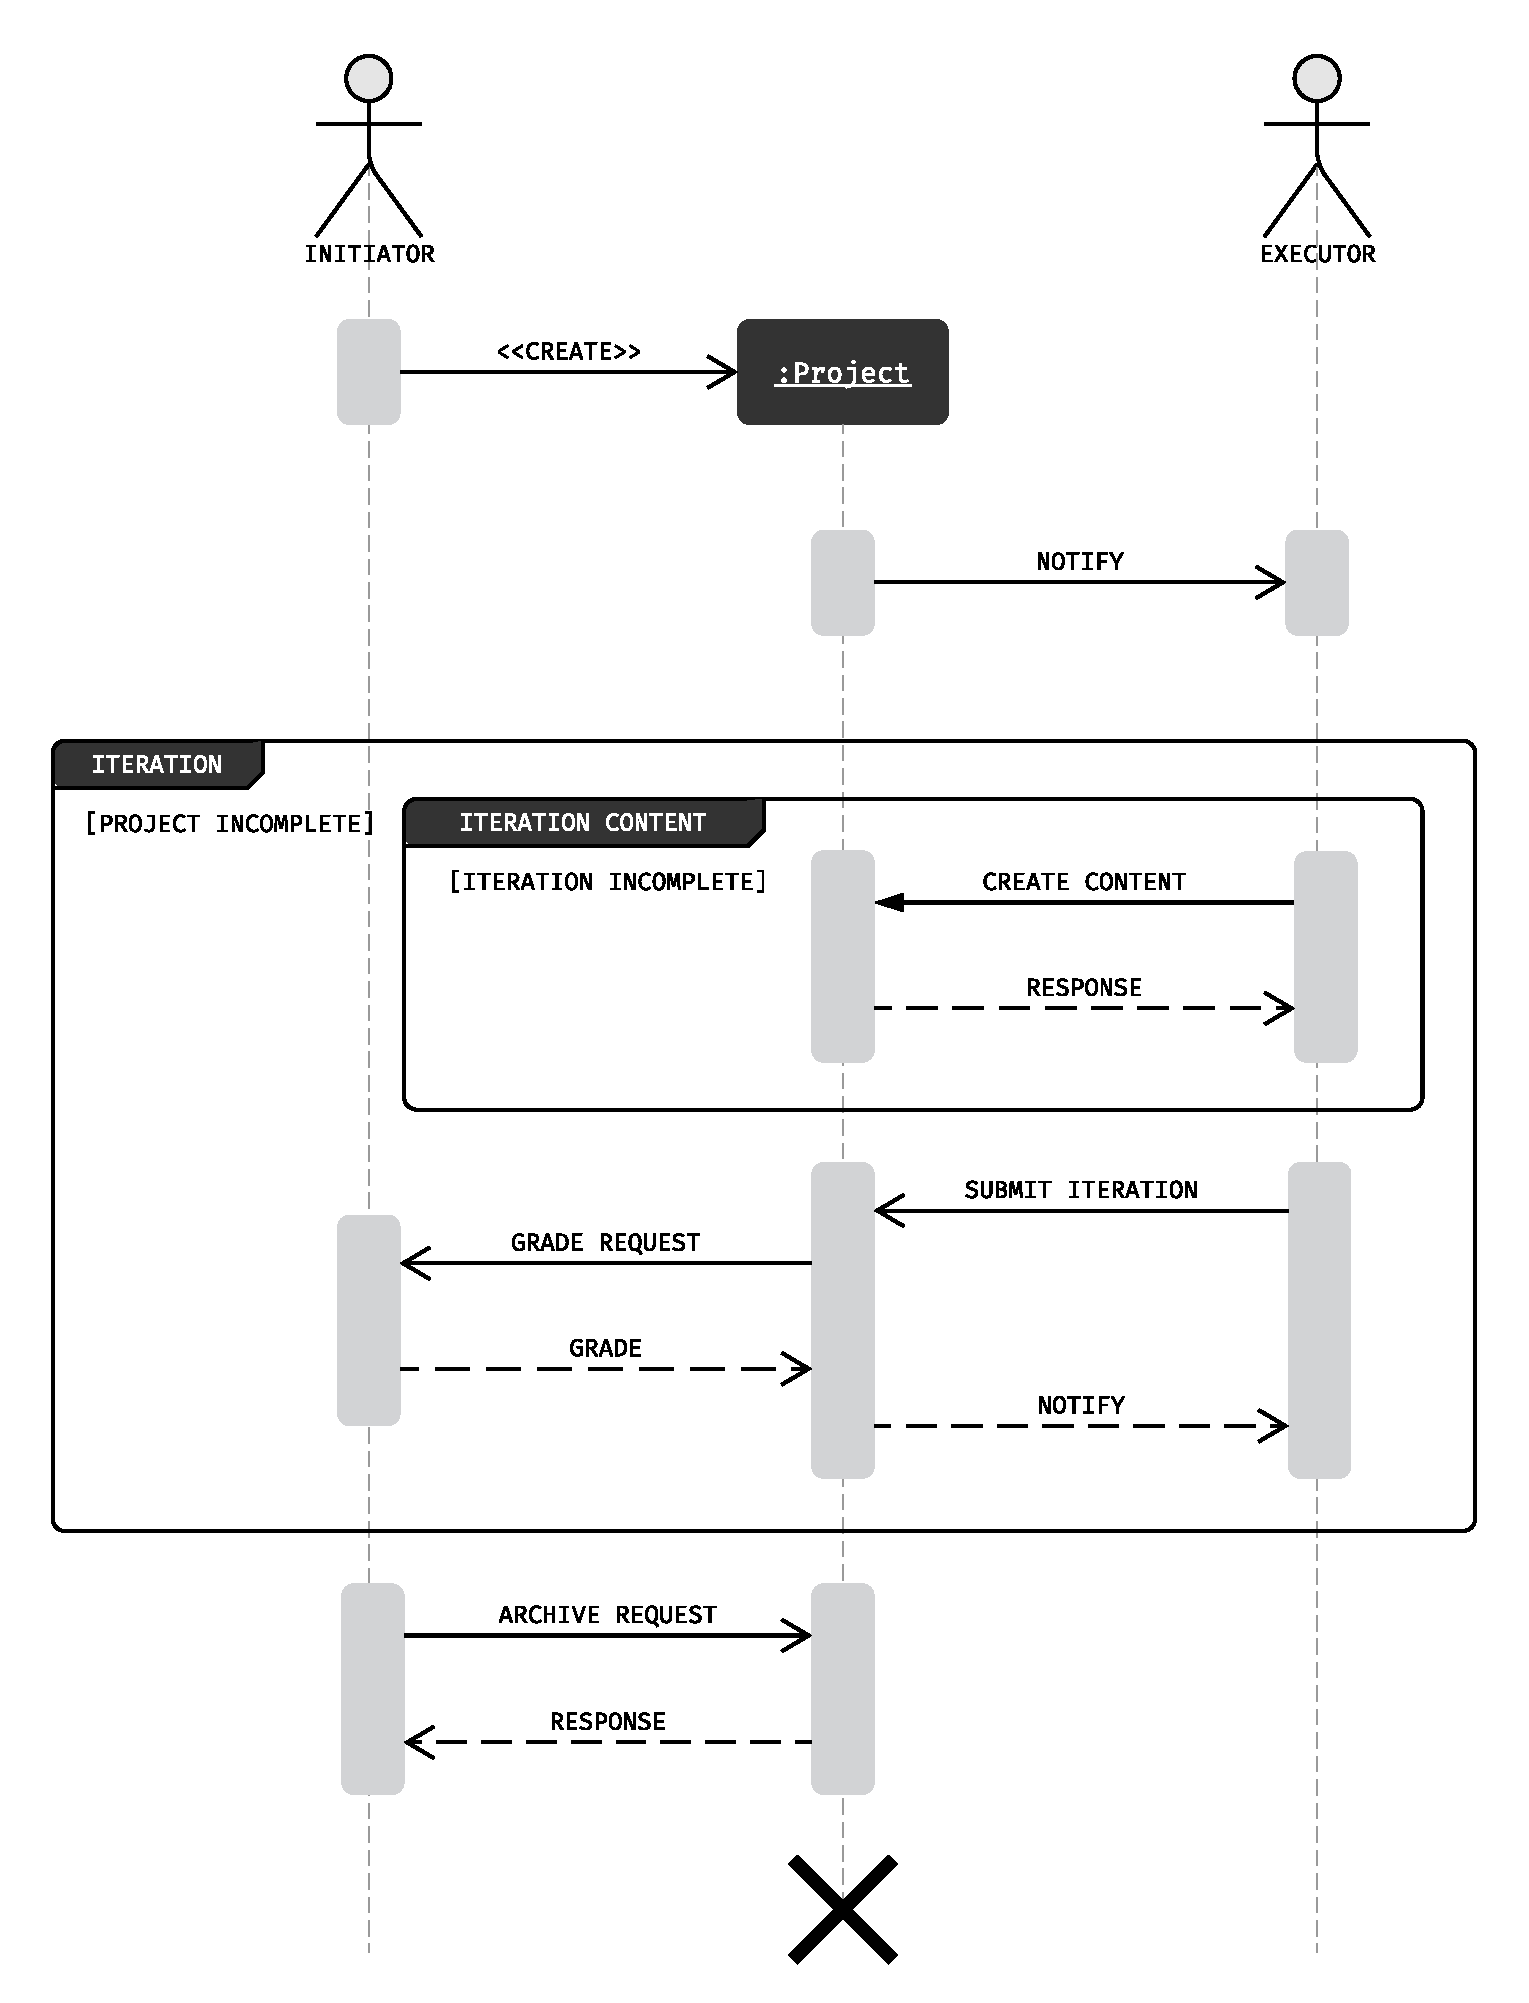
\includegraphics[max width=\textwidth]{assets/dia-seq-study-project-lifecycle}
   \caption[Zobecněný životní cyklus projektu]{Zobecněný životní cyklus projektu~\cite{bachelorthesis}}\label{fig:main-communication-cycle}
\end{figure}

\clearpage



\section{Základní požadavky a případy užití}\label{sec:required-spec}



\subsection{Funkční požadavky}\label{subsec:spec-req-func}

\begin{dl}
   \item[FP00]
   \textbf{Identita uživatelů} – uživatelé v systému jsou jednoznačně identifikovány a mohou vykonávat vykonávat určité činnosti na základě přidělených práv.
   \begin{dl}
      \item[FP00-UC00] Anonymní uživatel se může zaregistrovat.
      \item[FP00-UC01] Anonymní uživatel se může přihlásit.
      \item[FP00-UC02] Anonymní uživatel si může obnovit heslo dle emailu.
      \item[FP00-UC03] Přihlášený uživatel může vykonávat povolené operace dle práv.
   \end{dl}

   \item[FP01]
   \textbf{Globální role} – práva uživatelů jsou přidělována na základě rolí, administrátor systému má má neomezený přístup.
   Existuje 5 rolí: host (\h{guest}), uživatel (\h{user}), autorita (\h{authority}), administrátor (\h{admin}), zablokovaný uživatel (\h{banned}).
   \begin{dl}
      \item[FP01-UC00] \h{admin} může měnit uživatelům role.
      \item[FP01-UC01] \h{banned} má právo pouze na autentizaci, prohlížení osobních dat a odtranění.
   \end{dl}

   \item[FP02]
   \textbf{Uživatelská data} – aplikace umožňuje uživatelům prohlížet si svoje data a v případě nutnosti odstranit referenci na jejich osobu (odstranit účet).
   \begin{dl}
      \item[FP02-UC00] Přihlášený uživatel může prohlédnout svoje data uložená v systému.
      \item[FP02-UC01] Přihlášený uživatel může odstranit svůj účet.
   \end{dl}

   \item[FP03]
   \textbf{Upozornění} – aplikace posílá uživatelům relevantní upozornění na základě změn v \g{IS}.
   \begin{dl}
      \item[FP03-UC00] \h{user} může označit upozornění jako přečtené/nepřečtené.
      \item[FP03-UC01] \h{user} může odstranit upozornění.
   \end{dl}

   \item[FP04]
   \textbf{Projekt – životní cyklus} – aplikace umožňuje uživatelům zakládat projekty s definováním detailních interních informací.
   Projekt může být následně upravován až do jeho zániku (permanentní odstranění), nebo pozastavení (archivování na dobu neurčitou).
   \begin{dl}
      \item[FP04-UC00] \h{user} může založit projekt.
      \item[FP04-UC01] Pokud je projekt veden alespoň jedním \h{authority} uživatelem, tak je označen za důvěryhodný.
      \item[FP04-UC02] \h{user} s projektovou rolí \h{leader} může odstranit projekt.
      \item[FP04-UC03] \h{user} s projektovou rolí \h{leader} může archivovat projekt, nebo zrušit archivaci projektu.
   \end{dl}

   \item[FP05]
   \textbf{Projekt – správa dat} – aplikace umožňuje každému projektu definovat veřejná, skrytá (pouze pro účastníky projektu) a volitelně skrytá data.
   \begin{ul}
      \item \textbf{Veřejná} – kategorie, název, veřejný popis, cleny týmu, status archivace.
      \item \textbf{Skrytá} – interní popis.
      \item \textbf{Volitelně skrytá} – vakantní pozice, obsah.
   \end{ul}
   \begin{dl}
      \item[FP05-UC00] \h{user} s projektovou rolí \h{leader} může upravovat veškerá data.
      \item[FP05-UC01] \h{user} s projektovou rolí \h{leader} může upravovat viditelnost volitelně skytých dat.
      \item[FP05-UC02] \h{user} s projektovou rolí \h{contributor} může upravovat obsah.
      \item[FP05-UC03] \h{user} s projektovou rolí \h{visitor} může prohlížet skrytá data projektu.
   \end{dl}

   \item[FP06]
   \textbf{Projekt – kategorie} – aplikace umožňuje každému projektu definovat kategorie, dle kterých se dá vyhledávat.
   \begin{dl}
      \item[FP06-UC00] \h{admin} může zakládat a upravovat kategorie.
      \item[FP06-UC01] \h{admin} může odstranit kategorii, pokud neobsahuje ani jeden projekt.
   \end{dl}

   \item[FP07]
   \textbf{Projekt – tým a role} – v rámci každého projektu každý uživatel má určitou roli, která mu přiděluje oprávnění pro prohlížení/úpravu projektu.
   \begin{ul}
      \item
      \textbf{Vedoucí (\h{leader})} – neomezený přístup k projektu, spravuje všechny detaily projektu.
      Prvním vedoucím se stává uživatel, jenž projekt založil.
      \item
      \textbf{Spolupracovník (\h{contributor})} – podílí se na tvorbě obsahu projektu, nezasahuje do interní správy projektu.
      \item
      \textbf{Návštěvník (\h{visitor})} – může prohlížet skryté detaily projektu.
   \end{ul}
   Role Spolupracovník se nevyskytuje v projektu otevřeně, vedoucí projektu může definovat její podmnožiny, jako určité pozice v týmu s omezenou kapacitou.
   \begin{dl}
      \item[FP07-UC00] \h{user} s projektovou rolí \h{leader} může povolit/zakázat projektovou roli \h{visitor}.
      \item[FP07-UC01] \h{user} s projektovou rolí \h{leader} může definovat role v týmu, které jsou podskupinou projektové role \h{contributor}.
      \item[FP07-UC02] \h{user} s projektovou rolí \h{leader} může povolit/zakázat nábor do týmu.
      \item[FP07-UC03] \h{user} se může přihlásit na projektovou roli, pokud je povolený nábor a je volná kapacita role.
      \item[FP07-UC04] Účastník projektu může tým opustit, pokud se nejedná o posledního uživatele s projektovou rolí \h{leader}.
   \end{dl}

   \item[FP08]
   \textbf{Projekt – vyhledávání} – aplikace umožňuje vyhledat projekt dle zadaných kritérií.
   \begin{dl}
      \item[FP08-UC00] \h{user} s projektovou rolí \h{leader} může povolit nebo zakázat vyhledávání projektu.
      \item[FP08-UC01] \h{user} může vyhledat projekt dle kritérií, pokud je povoleno vyhledávání projektu.
   \end{dl}

   \item[FP09]
   \textbf{Projekt – Správa obsahu} – aplikace umožňuje vedoucím a spolupracovníkům tvořit obsah projektu.
   Obsah je členěn do částí – každá část má datovou složku a název interpretu, který bude danou datovou složku zpracovávat do vizuální podoby.
   \begin{dl}
      \item[FP09-UC00] \h{contributor} nebo \h{leader} projektu mohou vytvářet, upravovat a odstraňovat obsah.
      \item[FP09-UC01] \h{admin} může přidávat a odebírat dostupné globální interprety.
   \end{dl}
\end{dl}



\subsection{Obecné požadavky}\label{subsec:spec-req-common}

\begin{dl}
   \item[OP00]
   \textbf{Veřejné \g{API}} – aplikace bude nabízet veřejné i interní \g{API} s dokumentací pro vývoj mikroslužeb i klientských aplikací.

   \item[OP01]
   \textbf{Dokumentace} – součástí \g{IS} je uživatelská a vývojářská dokumentace.

   \item[OP02]
   \textbf{Rozšiřitelnost} – aplikace je přizpůsobena dalšímu rozvoji a umožňuje škálovat jednotlivé části funkcionality dle zátěže.

   \item[OP03]
   \textbf{Uživatelské rozhraní} – uživatelské rozhraní je ve webové podobě a podporuje prohlížeč Google Chrome.
   Mobilní rozhraní není potřeba.

   \item[OP04]
   \textbf{Jazykové verze} – rozhraní je připraveno pro překlad do dalších jazyků.

   \item[OP05]
   \textbf{Úložiště dat projektů} – úložiště dat projektů bude možné měnit před prvním spuštěním \g{IS}.
   Výměna úložiště se zachováním údajů během provozu \g{IS} není nutná.
\end{dl}


\clearpage



\section{Rozvojové požadavky a případy užití}\label{sec:optional-spec}


\begin{dl}
   \item[FP10]
   \textbf{Projekt – tagy} – aplikace umožňuje každému projektu definovat veřejné tagy, dle kterých se dá vyhledávat.
   \begin{dl}
      \item[FP06-UC00] Tag vzniká během založení nebo úpravě projektu.
      \item[FP06-UC01] \h{admin} může upravovat název tagu.
      \item[FP06-UC02] \h{admin} může odstranit tag, pokud ho nevyužívá ani jeden projekt.
   \end{dl}


   \item[FP11]
   \textbf{Projekt – iterace a úkoly} – projekt může být rozdělen na jednotlivé iterace, které se skládají z jednoho, nebo více úkolů.
   Jednotlivé části obsahu projektu mohou tyto úkoly označovat jako splněné.
   \begin{dl}
      \item[FP09-UC00] \h{leader} projektu může založit projekt s iteracemi, nebo přidat iterace do existujícího projektu.
      \item[FP09-UC01] \h{leader} projektu může upravovat iterace a úkoly.
      \item[FP09-UC01] \h{leader} projektu může odstraňovat iterace a úkoly, pokud nejsou spjaty s existujícím ohodnocením.
      \item[FP09-UC02] Uživatelé tvořící obsah mohou označovat jednotlivé úkoly jako splněné u každé části obsahu.
   \end{dl}


   \item[FP12]
   \textbf{Projekt – snímky iterací} – stav obsahu projektu se dá zafixovat a kdykoliv prohlédnout.
   Tento stav bude neměnným historickým milníkem všech částí obsahu, u něhož je rovněž uložena informace ohledně autora snímku, splněných iterací a úkolů.
   \begin{dl}
      \item[FP11-UC00] \h{leader} nebo \h{contributor} projektu může z aktuálního stavu projektu vytvořit snímek.
      \item[FP11-UC01] Účastník projektu může prohlédnout jakýkoliv historický snímek projektu.
   \end{dl}


   \item[FP13]
   \textbf{Projekt – hodnocení iterací} – odevzdané iterace (snímky iterací) se dají ohodnotit body.
   Každý úkol má minimální požadovaný a maximální počet bodů, kterými může být ohodnocen.
   Ke každému ohodnocení úkolu a iterace lze doplnit komentář.
   \begin{dl}
      \item[FP11-UC00] \h{leader} nebo \h{contributor} projektu může u snímku vyžádat ohodnocení ze strany jednoho z uživatelů typu \h{authority} s projektovou rolí \h{leader}.
      \item[FP11-UC01] \h{authority} s projektovou rolí \h{leader} může ohodnotit odevzdanou iteraci.
      \item[FP11-UC02] \h{authority} s projektovou rolí \h{leader} může upravit svoje vlastní ohodnocení.
   \end{dl}

   \item[FP14]
   \textbf{Projekt – Editace týmu} – tým lze nabírat nejen z dobrovolníků, ale i striktním přiřazováním uživatelů.
   \begin{dl}
      \item[FP11-UC00] \h{authority} s projektovou rolí \h{leader} může do týmu projektu přidávat účastníky bez jejich souhlasu.
   \end{dl}
\end{dl}
